%priprava posamezne ure
%tukaj zaporedoma napisemo{st. zaporedne ure}{datum}{naslov}{poglavje}{oblika dela}{pripomocki}
\begin{priprava}{}{}{Limita funkcije}{Limita funkcije}{frontalna}{tabla}

\didopomba{Pojem limite in okolice so spoznali že v zaporedjih, tako da ne preveč čarati tukaj, da se ne zmedejo. Limita zanje pomeni približevanje zaporedja/funckije neki vrednosti, ko gre $n, x $ ali katerakoli druga spremenljivka nekam.}

Poglejmo si tri primere funkcije:

\begin{figure*}[h]
    \centering
    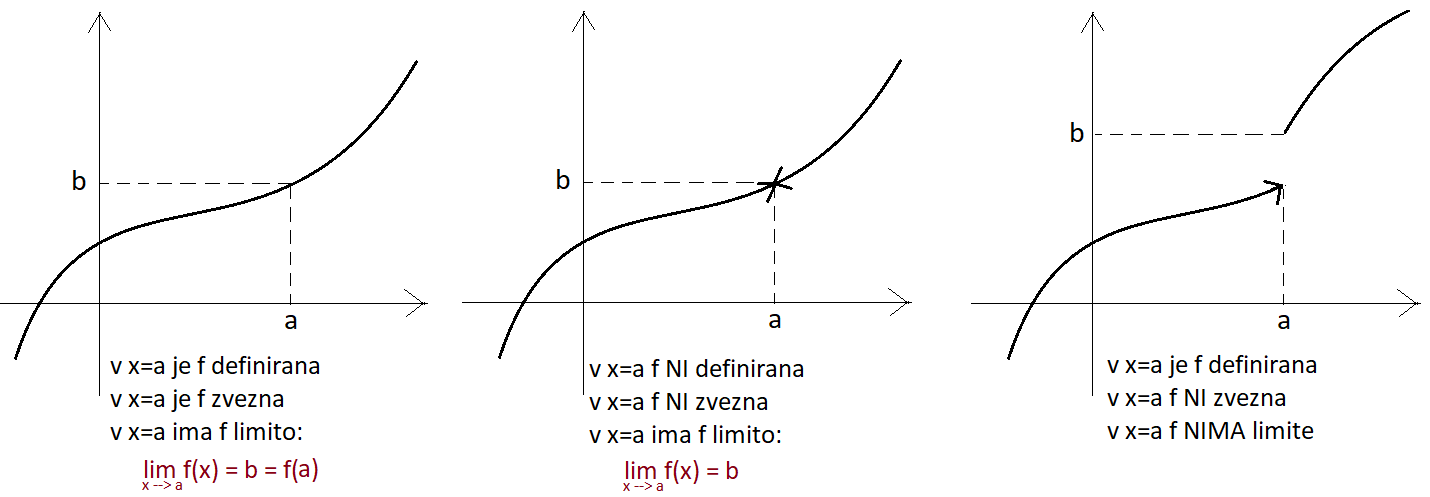
\includegraphics[width=\textwidth]{slike/limita.png}
\end{figure*}

Število $ b $ je \textbf{limita funkcije} $ f $ v točki $ a $, če za vsak $ x $ iz okolice $ a $ velja, da so funkcijske vrednosti v izbrani okolici $ b $.

\begin{figure*}[h]
    \centering
    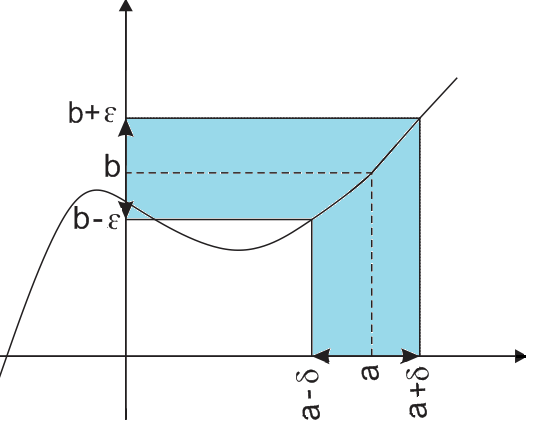
\includegraphics[width=0.4\textwidth]{slike/limita_okolice.png}
\end{figure*}

\didopomba{pri tretji slikci za majhno okolico $ b $-ja vsaka vrednost $ f $ levo od $ a $ pade ven iz te okolice, zato tam limita ne obstaja.}

\didopomba{Meni se ne zdi potrebno, da jih matramo s temi epsiloni in deltami :D }

\didopomba{dopolnimo definicijo zveznosti:}

Funckija je \textbf{zvezna} v $ a $, če je v $ a $ definirana in ima limito. Limita je v tem primeru kar vrednost $ f $ v $ a $ -- $ f(a) $. \didopomba{prvi primer iz slikice}

\newpage

\textbf{Računanje z limitami:} \didopomba{intuitivno, saj veljo enako kot za zaporedja}
\begin{itemize}
    \item $ \lim_{x \to a} (f(x) + g(x)) = \lim_{x \to a} f(x) + \lim_{x \to a} g(x) $
    \item $ \lim_{x \to a} (f(x) \cdot g(x)) = \lim_{x \to a} f(x) \cdot \lim_{x \to a} g(x) $
    \item $ \lim_{x \to a} \frac{f(x)}{g(x)} = \frac{\lim_{x \to a} f(x)}{\lim_{x \to a} g(x)} $, če $ \lim_{x \to a} g(x) \neq 0 $
    \item $ \lim_{x \to a} (k \cdot f(x)) =  k \cdot \lim_{x \to a} f(x) $
    \item $ \lim_{x \to a} c = c $
\end{itemize}

Kako računati npr. $ \lim_{x \to 3} x + 8 $?
\begin{enumerate}
    \item Najprej poskusi vstaviti vrednost.
    \item Če v imenovalcu dobiš 0, poglej, ali se da kaj okrajšati z razstavljanjem ali razširjanjem
\end{enumerate}

\vaje{
Vaje:
\begin{itemize}
    \item Enostavne naloge, kjer samo vstavijo vrednost noter in izračunajo
    \item primeri, kjer imenovalec pride 0, ampak se problematični deli okrajšajo, ko uporabimo npr. Vietovo pravilo, razliko kvadratov, racionaliziramo števec
\end{itemize}
}

Kaj lahko poveš o funkciji, če veš, da: \didopomba{naj sami razmislijo}
\begin{itemize}
    \item $ \lim_{x \to a} f(x) = f(a) \to f $ je zvezna v $ a $
    \item $ \lim_{x \to \infty} f(x) = a \to f $ ima vodoravno asimptoto $ y = a $ \didopomba{slikca!}
    \item $ \lim_{x \to a} f(x) = \infty $ ali $ - \infty \rightarrow f $ ima v $ a $ pol sode stopnje (pri polu lihe stopnje limita ne obstaja)
\end{itemize}
    
\textbf{Limita trigonometrijske funkcije:}

najprej nekaj limit, kjer se vseeno da vstaviti in ni problema. Potem pa problem: $ \lim_{x \to 0} \frac{\sin {3x}}{5x} $, kaj pa tu?

\begin{figure*}[h]
    \centering
    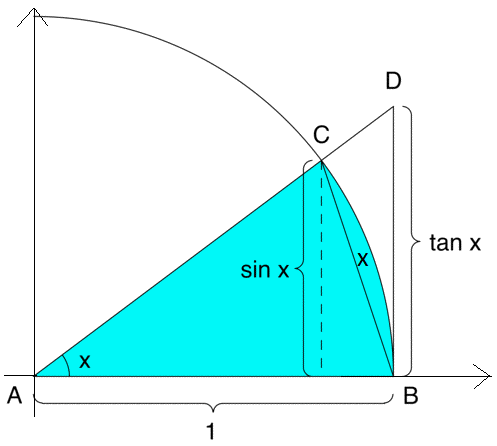
\includegraphics[width=0.5\textwidth]{slike/limita_sin.png}
\end{figure*}

\newpage

\begin{align*}
    \sin x < & x < \tan x \; / : \sin x \\
    1 < & \frac{x}{\sin x} < \frac{1}{\cos x} \; / ^{-1} \\
    \cos x < & \frac{\sin x}{x} < 1 \; / lim_{x \to 0} \\
    lim_{x \to 0} \cos x < & lim_{x \to 0} \frac{\sin x}{x} < lim_{x \to 0} 1 \\
    1 < & lim_{x \to 0} \frac{\sin x}{x} < 1
\end{align*}

Sledi $ lim_{x \to 0} \frac{\sin x}{x} = 1 $ \didopomba{Lahko pokažeš slikco $ \frac{\sin x}{x} $}

\begin{figure*}[h]
    \centering
    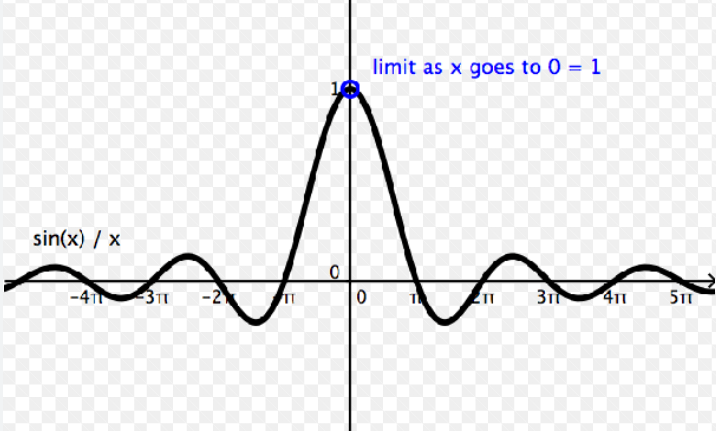
\includegraphics[width=0.7\textwidth]{slike/limita_sin2.png}
\end{figure*}

\vaje{Še nekaj vaj, kjer se to uporabi, tudi na problemu (razširiš števec in imenovalec z argumentom v sinusu), upoštevaš trigonometrične lastnosti npr. dvojni koti ipd.}
\end{priprava}